\chapter{Stability \& Control}
\label{sec:manostab}

Regardless of performance characteristics, controlling the vehicle is of vital importance to any mission at any phase. For the aircraft under consideration, the controllability is absolutely crucial in both vertical and in horizontal flight. Horizontal flight phases for this particular vehicle are associated with high velocities at low altitudes, which requires very precise control of the UAV. Vertical flight phases are associated with taking off and landing on small landing sites possibly in an urban environment. In this condition the allowed attitude and positional errors are expected to be very limited. In order to ensure that these aspects are sufficiently and correctly represented in the selection process, all concepts are analysed for manoeuvrability, stability and controllability in this chapter. First, the results of this analysis are summarised in \autoref{sec:sum}. Then, the general approaches for judging  manoeuvrability, stability and controllability as well as the assigned weights are explained in \autoref{sec:app}. Finally, the reasoning behind each rating is explained in more detail per sub criterion and per concept in \autoref{sec:ca}.

\section{Summary}
\label{sec:sum}

The final result of the analysis performed in this chapter is summarised in \autoref{tab:controlsubtrade}:

\begin{table}[H]
    \centering
    \caption{MSC Sub Trade-off}
    \label{tab:controlsubtrade}
    \begin{tabular}{r|>{\centering}p{4cm}:>{\centering}p{3.5cm}:>{\centering}p{2.5cm}|c}
    \textbf{Concept \rotatebox{90}{\hspace{0.5cm}Criterion}}    & 
    \rotatebox{90}{\textbf{Controllability}}                      &
    \rotatebox{90}{\textbf{Stability}}                           & 
    \rotatebox{90}{\textbf{Manoeuvrability}}  &  
    \rotatebox{90}{\textbf{Outcome}}                    
    \\ \midrule
    Tailsitter      & -   & 0   & +   & 46\% 
    \\\hdashline
    Tandem          & 0     & -     & 0      & 41\% 
    \\\hdashline
    Prandtl Box     & 0     &  -   & 0     & 41\% 
    \\\hdashline
    Tiltrotor       &  + +     & +   & -   & 72\% 
    \\\hdashline
    Winged Quad.     & + +    & +     & +    & 85\% 
    \\ \midrule\midrule
    Weight          & 40    & 35    & 25    &  
    \end{tabular}
\end{table}

As can be seen, the highest score was earned by the Winged Quadcopter. It combines good controllability in both horizontal and vertical flight modes with a relatively wide range of allowable CG locations for stability and more manoeuvrability than most other concepts. The Tiltrotor concept earned the second highest score in this sub trade-off. Its score is identical to that of the Winged Quadcopter in both the controllability and stability departments. However, it does score lower on manoeuvrability due to its high moments of inertia about the X and Z axes. These higher moments of inertia can be contributed to the placement of the engines, which both are at the wing tips. The Tailsitter was ranked third with a score of 46.25 \% . The main reasons for this lower score were the relatively limited range of CG positions for stability and the lower control surface effectiveness. In manoeuvrability, the concept performed comparable to the Winged Quadcopter. The Tailsitter is closely followed by the Tandem and Prandtl Box concepts, which both scored 41.25 \%. They both have a limited range of allowable CG positions for stability whilst neither score particularly high in controllability nor in manoeuvrability.

\section{Approach}
\label{sec:app}


\subsection{Reference Frame}

In order to have a consistent axis system throughout the report, the right-handed, body-fixed reference frame $F_b$ was chosen as a basis. It is visualised in \autoref{fig:body_frame}. 

\begin{figure}[htb]
    \centering
    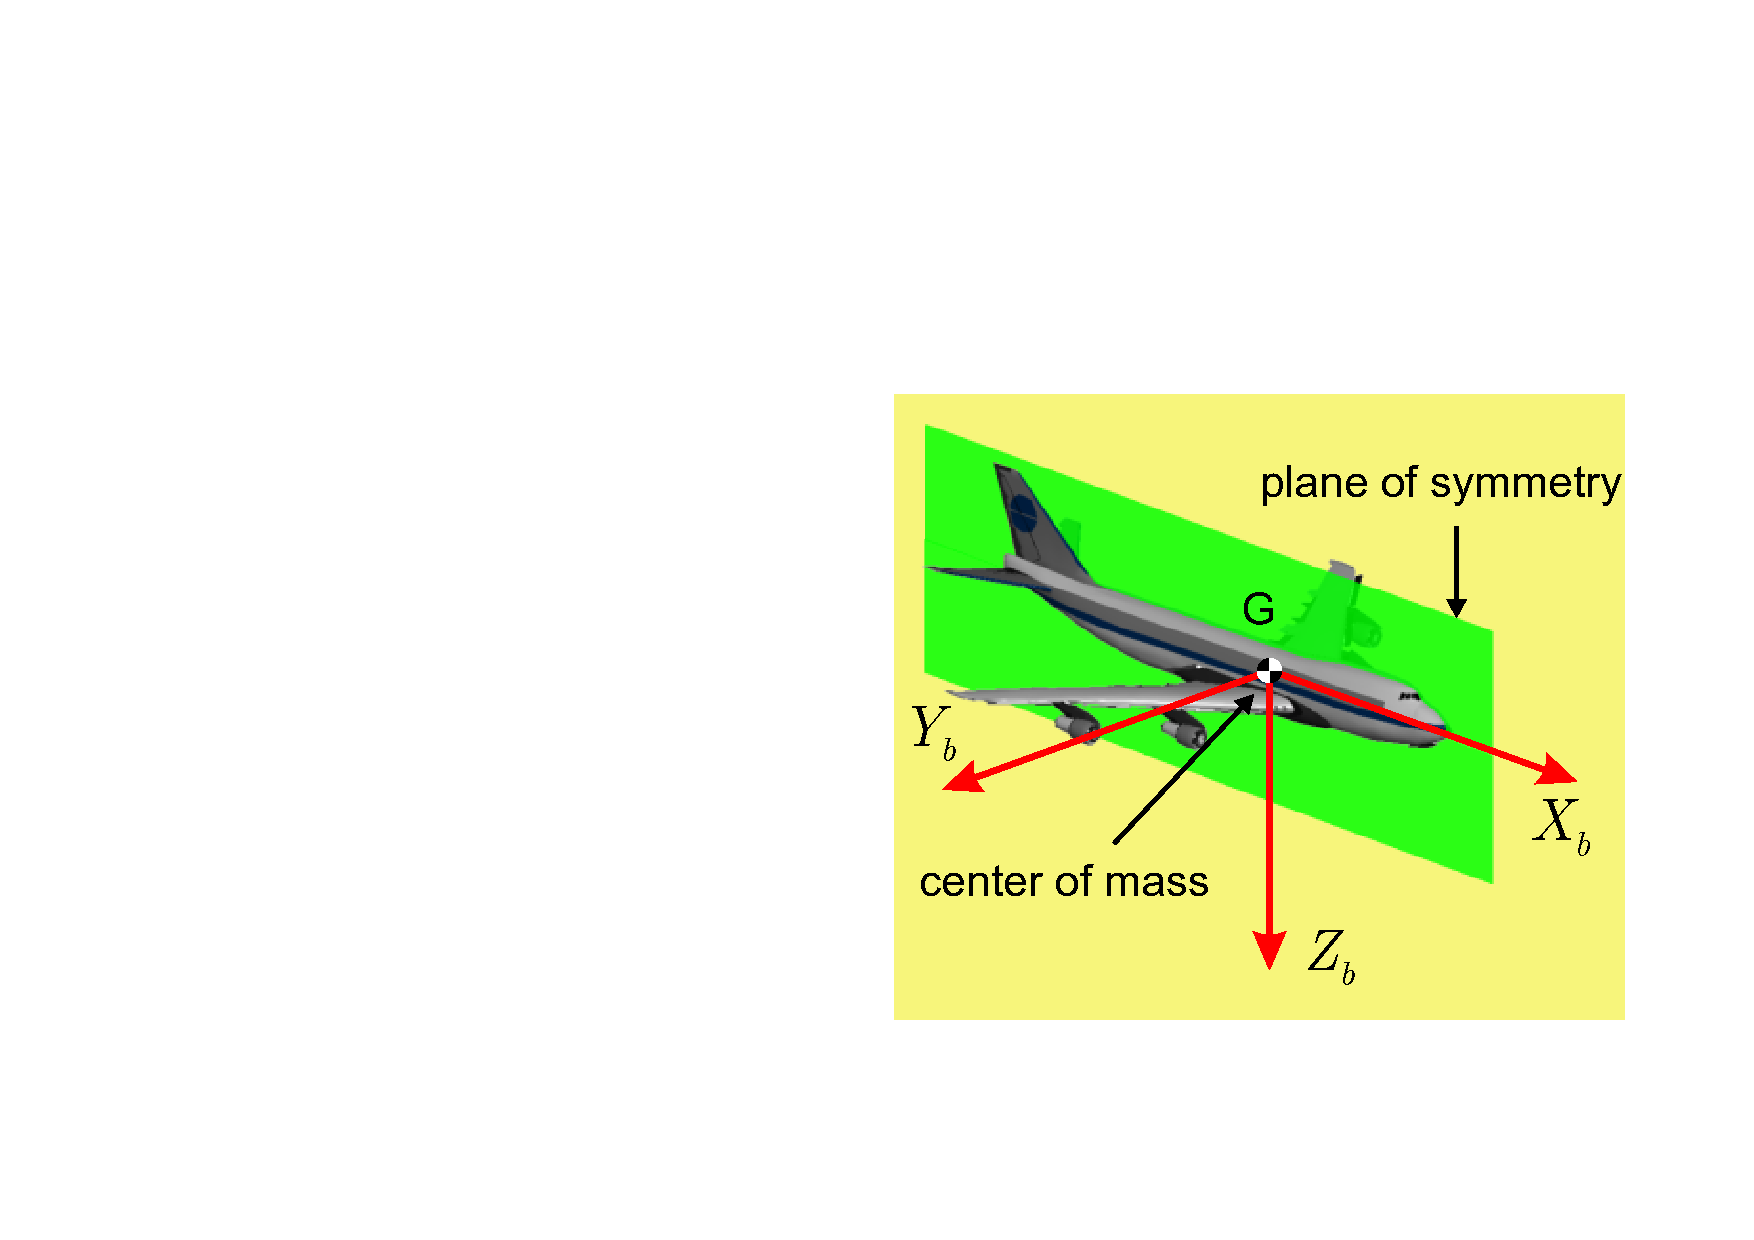
\includegraphics[width=.35\textwidth]{Stability/Figures/body_frame.pdf}
    \caption{Body Fixed Reference Frame \cite{fd_lec08}}
    \label{fig:body_frame}
\end{figure}



\subsection{Stability}

The stability of each concept in both horizontal and vertical flight regimes was investigated based on the sketches available from the Baseline Report \cite{baseline}. For horizontal flight the configurations of the lifting surfaces were evaluated for the change in pitching moment due to a disturbance change in angle of attack. The range of Centre of Gravity (CG) locations for which the aircraft would be longitudinally stable was evaluated per concept. For vertical flight stability, the configuration of the engines is evaluated because none of the concepts employ lifting surfaces in this mode. The definition of the scores can be found below in \autoref{tab:dsr}. 

\begin{table}[H]
\centering
\caption{Definition of Stability Ratings}
\label{tab:dsr}
    \begin{tabular}{llc}
        \toprule
            &\textbf{Rating}           & \textbf{Meaning}
        \\ \midrule
          & ++            & Stable in horizontal and vertical flight for a wide range of CG positions          
        \\ \hdashline
          & +               & Stable for wide CG range in horizontal flight, neutrally stable in vertical flight
        \\ \hdashline
          & 0          & Stable in horizontal flight for limited CG range, stable in vertical flight 
        \\ \hdashline
          & -           & Stable in horizontal flight for limited CG range, neutral stability in vertical flight 
        \\ \hdashline
          & - -   & Unstable in horizontal or vertical flight
        \\ \bottomrule
    \end{tabular}
\end{table}

\subsection{Controllability}

The control systems of the different concepts were analysed for their effectiveness based on the moment arms for various control surfaces and engines as derived from the geometry of the conceptual sketches. The definitions of the ratings are shown in \autoref{tab:dcr}.

\begin{table}[H]
\centering
\caption{Definition of Control Ratings}
\label{tab:dcr}
    \begin{tabular}{llc}
        \toprule
            &\textbf{Rating}           & \textbf{Meaning}
        \\ \midrule
          & ++            &  Effective pitch, roll and yaw control      
        \\ \hdashline
          & +               & Effective pitch control,low roll and yaw control effectiveness
        \\ \hdashline
          & 0          & Average pitch control effectiveness
        \\ \hdashline
          & -           & Low pitch control effectiveness, effective roll control
        \\ \hdashline
          & - -    & Low pitch and roll control effectiveness
        \\ \bottomrule
    \end{tabular}
\end{table}

\subsection{Manoeuvrability}

Next to the control surface effectiveness it is desirable to have a low mass moment of inertia around all three body axes. Even though the Hybrid UAV will be optimised for high-speed cruise conditions, it still needs to be able to roll and pitch up quickly, for instance, to avoid obstacles at low altitudes.

The approach to analysing the moments of inertia was to use the weight and wing size estimations derived in \autoref{ch:perf_analy} to create simplified CATIA models of each concept. Since the knowledge about geometry and component weights is limited at this stage of the project, a number of assumptions are made. The most important ones are listed below:

\begin{itemize}%leave periods in this table -K
    \item All concepts share the same cylindrical fuselage which includes battery and payload.
    \item Engines and propellers can be modelled as a single cylinder and have a constant power-to-weight ratio.
    \item Engine mass is 20\% of total mass (based on a statistical analysis in \cite{Wei_2017}).
    \item Horizontal and vertical tail plane surfaces are 20\% of the main wing area (based on ratios derived from reference aircraft \footnote{\url{https://booksite.elsevier.com/9780340741528/appendices/data-a/table-8/table.htm}}).
    \item Structural mass per unit area is equal for all aerodynamic surfaces.
\end{itemize}

\autoref{fig:prandtl_inertia} shows the model of the Prandtl Box concept to give an impression of the level of accuracy that can be achieved by this analysis. Since the fuselage and payload is assumed to be equal for all five concepts, the main differences in inertia follow from the area and aspect ratio of the wing, mass and placement of the engines and the presence of additional elements such as tailplanes and wing connectors. Even though the absolute value of the result should be handled with care and updated when more reliable dimensions and mass values are available, the distinct configuration of each concept allows for a reasonable comparison. 

\begin{figure}[htb]
    \centering
    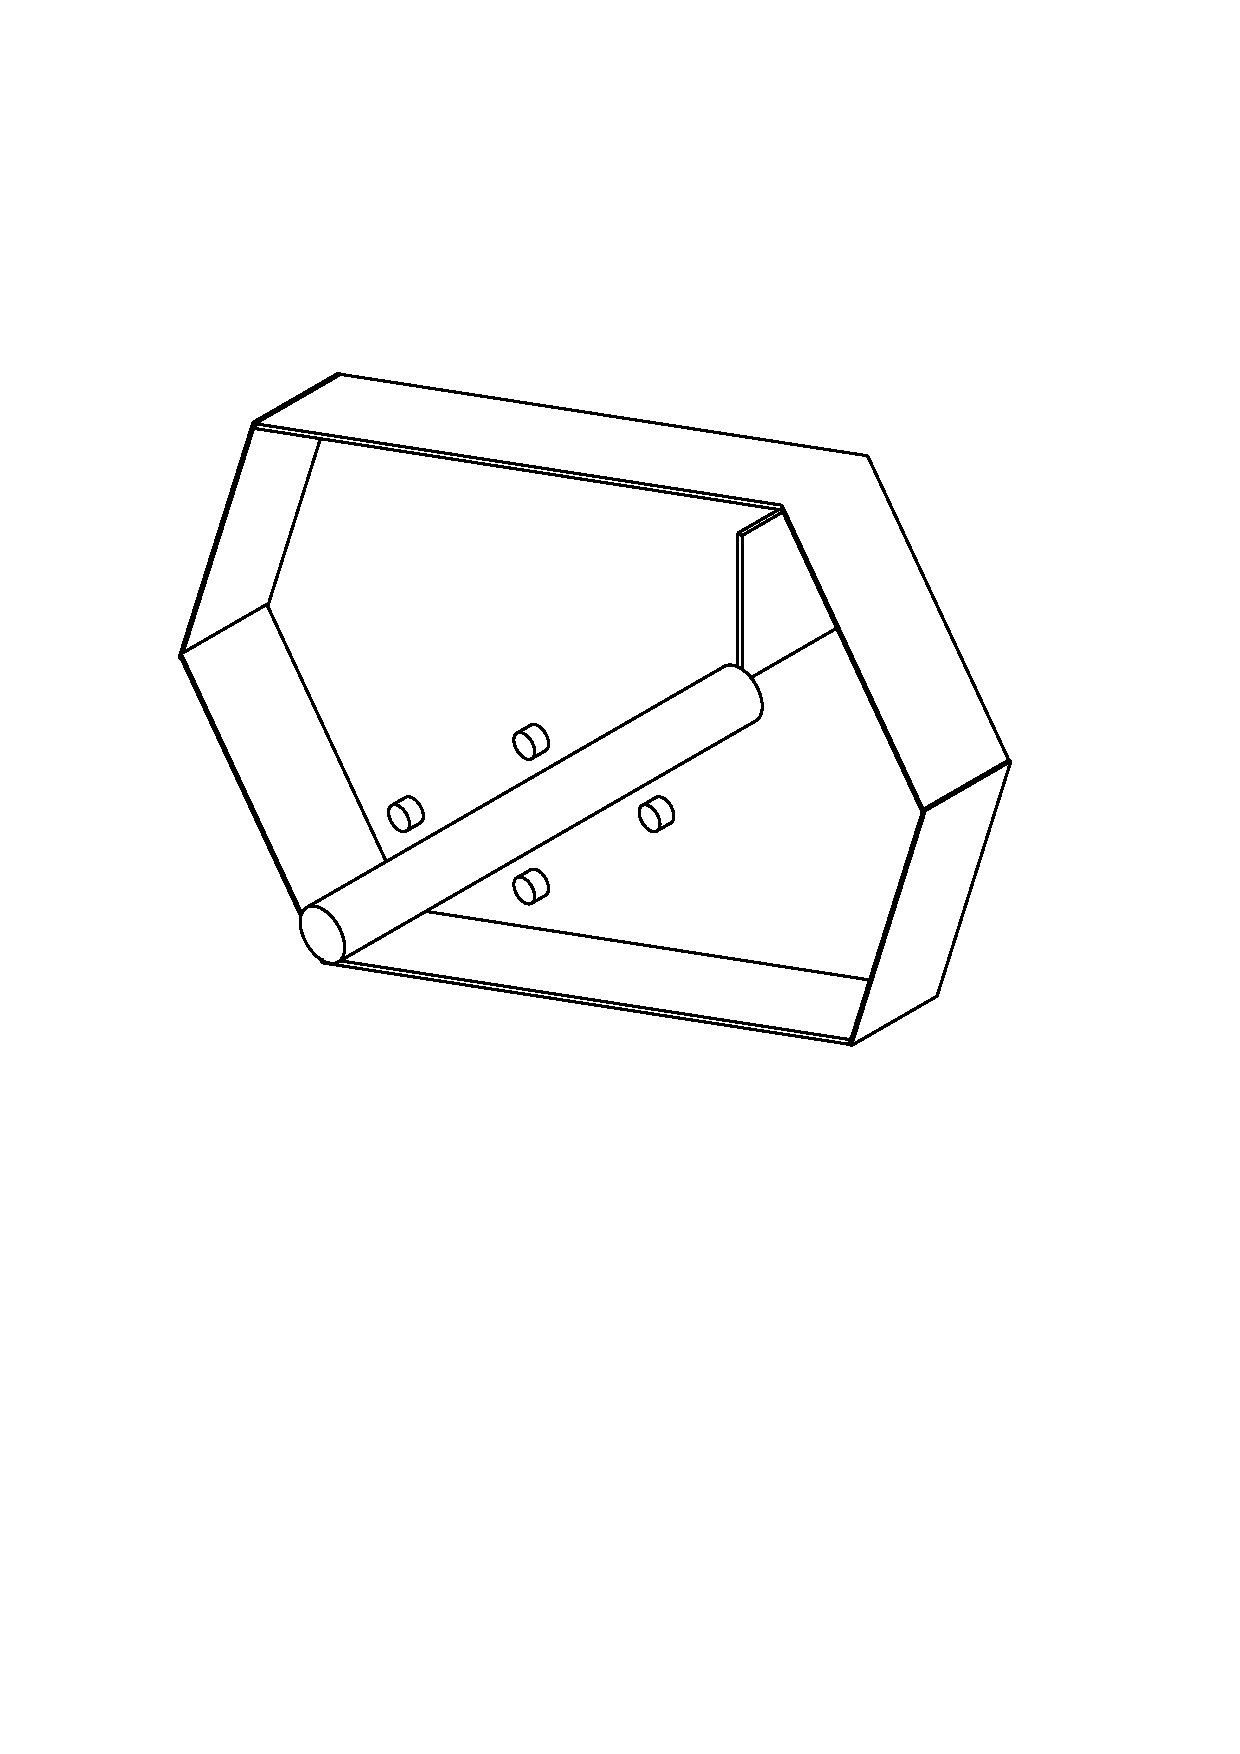
\includegraphics[width=.4\textwidth]{Stability/Figures/prandtl.pdf}
    \caption{Simplified Model of the Prandtl Box Concept}
    \label{fig:prandtl_inertia}
\end{figure}

\autoref{tab:dmr} shows the rating scheme for manoeuvrability, it is derived by doubling the average total inertia of all concepts and then splitting the resulting range into five categories.  

\begin{table}[H]
\centering
\caption{Definition of Manoeuvrability Ratings}
\label{tab:dmr}
    \begin{tabular}{llc}
        \toprule
            &\textbf{Rating}           & \textbf{Total inertia range $[kg \times m^2]$}
        \\ \midrule
          & ++            &  0-30       
        \\ \hdashline
          & +               & 30-60
        \\ \hdashline
          & 0          & 60-90
        \\ \hdashline
          & -           & 90-120
        \\ \hdashline
          & - -    & 120 and more
        \\ \bottomrule
    \end{tabular}
\end{table}

\subsection{Criteria Weights}
In order of increasing importance the sub criteria are as following: manoeuvrability, stability and control. Their weights are determined to be 25, 35 and 40 respectively. Manoeuvrability is assigned the lowest weight out of the three criteria because good manoeuvrability is less vital for the UAV's intended mission. Control is weighted heavier than stability because an effective control system can overcome the undesirable effects of an unstable aircraft, whereas an ineffective control system paired with a very stable aircraft becomes even more of a problem. 

% Oscar: Tailsitter
\section{Concept Analysis}
\label{sec:ca}

All five concepts were analysed for their controllability, stability and manoeuvrability. As was explained in \autoref{sec:app}, the values obtained for moments of inertia are most meaningful in comparison, so a table was added in the beginning. 

\subsection{Overview of Mass Moments of Inertia}

\autoref{tab:inertia_overview} shows the result of the MOI analysis for all concepts. A brief discussion of remarkable values is provided in the concept sections. 

\begin{table}[htb]
    \centering
    \caption{Mass Moments of Inertia for Each Concept in $[kg \times m^2]$ }
    \label{tab:inertia_overview}
    %\begin{adjustbox}{width=1\textwidth}
    \small
        \begin{tabular}{lcccc}
        \toprule
        \textbf{Concept} & \textbf{$I_x$} & \textbf{$I_y$} & \textbf{$I_z$} & \textbf{$I_{total}$} \\ \midrule
        The Tailsitter          &1.9   & 25.3  & 26.6 & 53.7    \\\hdashline
        The Tandem              &10.0  & 27.3  & 36.3 & 73.6    \\\hdashline
        The Prandtl Box         &13.6  & 26.4  & 35.1 & 75.1    \\\hdashline
        The Tiltrotor           &32.7  & 23.5  & 53.9 & 110.1   \\\hdashline
        The Winged Quad.        &4.9   & 20.3  & 24.2 & 49.4    \\\bottomrule
        \end{tabular}
        %\end{adjustbox}
\end{table}

\subsection{The Tailsitter}
\begin{figure}[htb]
    \centering
    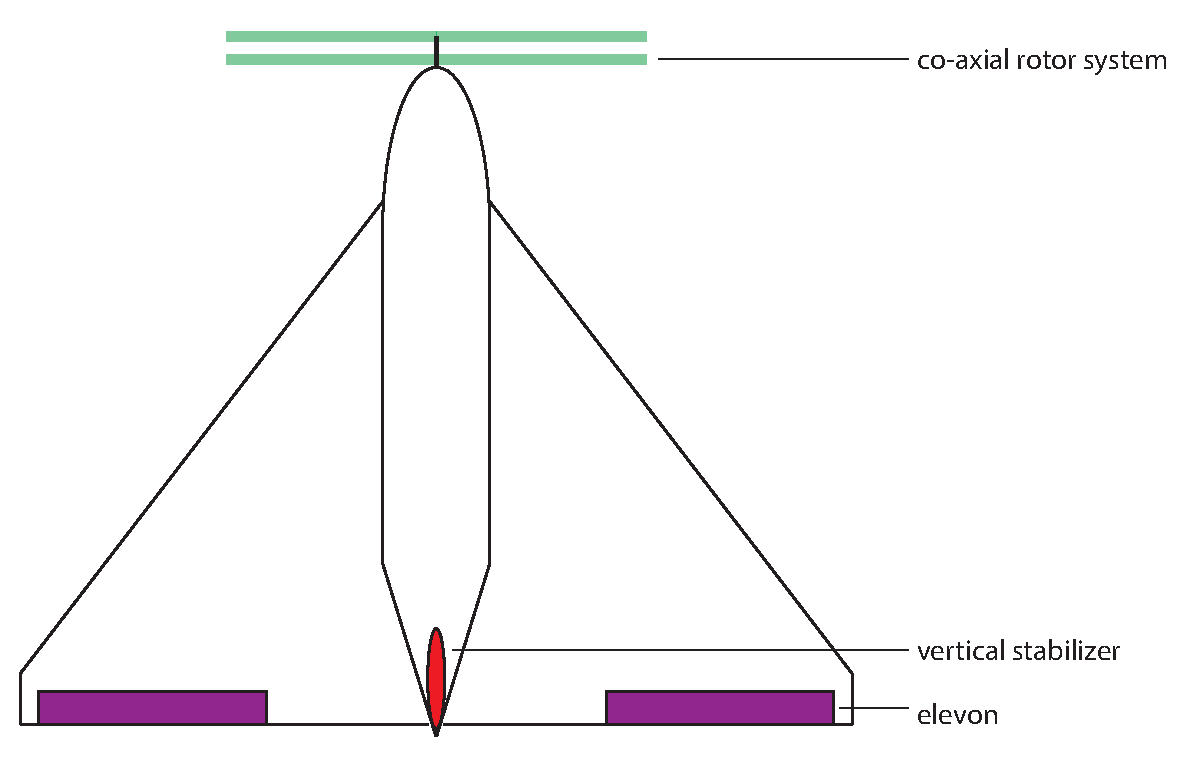
\includegraphics[height=6cm]{Stability/Figures/concept_1.pdf}
    \caption{Control Layout of The Tailsitter.}
    \label{fig:Cts}
\end{figure}
\paragraph{Control}

The layout of the control system for the Tailsitter is depicted in \autoref{fig:Cts}. In vertical flight mode, the attitude of the Tailsitter is fully controlled with the coaxial rotors mounted on the nose of the aircraft. As they are counter rotating, the yaw rate of the vehicle can be controlled by inversely adjusting the angle of attack of both the rotor blades. Additionally, both the pitch and roll rates can be manipulated with cyclic angle of attack increments on both rotors. Finally, the rate of ascent or decent is controlled with collective angle of attack adjustments on both rotors. 

In horizontal flight phases, the coaxial rotors are only used as a means of propulsion. Attitude control is achieved solely by the manipulation of aerodynamic control surfaces. Particularly, a conventional rudder is used for directional control and both longitudinal and lateral control are accomplished with a single set of control surfaces. These elevons are located at the trailing edge of the delta-shaped wing.

Because this design lacks a conventional tail, the aerodynamic control surfaces used to generate the required pitching moments are located closer to the centre of gravity than for conventional aircraft. This means that either larger surfaces or greater deflection angles are required to generate a sufficient pitching moment. Consequently, the trim drag will be higher for this concept than for a standard configuration aircraft. Similarly, the rudder is also located closer to the centre of gravity in this configuration. Hence, for the rudder to be effective, a rather large surface or a significantly larger deflection of this surface are required. This will increase the amount of drag associated with use of the rudder. However, the propellers are mounted on the aircraft's centre line. Therefore, no prolonged rudder deflections are required to balance out a propulsion induced torque in a one engine out scenario. Furthermore, take-off and landing are performed in vertical mode without use of the control surfaces. So, the rudder is not frequently used during flight and its lower efficiency is therefore tolerable. The increased trim drag that is sustained for longitudinal stability might be detrimental to the performance of this design. 


\paragraph{Manoeuvrability}

The Tailsitter is a very promising concept when it comes to manoeuvrability. The engine block and propellers are situated on the centre line of the UAV, meaning that there is no extra inertia term due to axis offsets in y and z direction. In combination with low wing span, this leads to a very low moment of inertia around the roll axis compared to the other concepts. The MOIs around the pitch and yaw axis are average, which is due to the large wing surface and the offset of the engine to the UAV c.g. in x direction. 

\paragraph{Stability}

In vertical flight mode, The Tailsitter is neutrally stable about all three axes. The centre of gravity always lies on the line of action of the thrust force, because of the way the rotors are mounted on the vehicle. Furthermore, the gravitational force vector goes through the centre of gravity by definition. Hence, a disturbance to any equilibrium condition is neither amplified nor restored. The stability could be improved by employing a stabiliser bar, as is quite common in helicopter designs. On the other hand the lack of stability could be overcome with active control such an electronic control unit based on gyroscopic sensors.

During horizontal manoeuvres, the tailless delta wing configuration is not ideal from a stability point of view. The vehicle has only a single lifting surface. Therefore in order to have longitudinal stability, the centre of gravity should be in front of the aerodynamic centre and the moment about the aerodynamic centre should be positive. This imposes some limitations on the weight distribution and wing design. High-camber airfoils or trailing edge high-lift devices contribute to a negative pitching moment about the aerodynamic centre. Their application would therefore adversely affect the stability of the UAV. On the contrary, implementing a wash-out or a reflex cambered airfoil as an example would increase the pitching moment about the aerodynamic centre.

%Oscar: Tandem
\subsection{The Tandem}
\begin{figure}[htb]
    \centering
    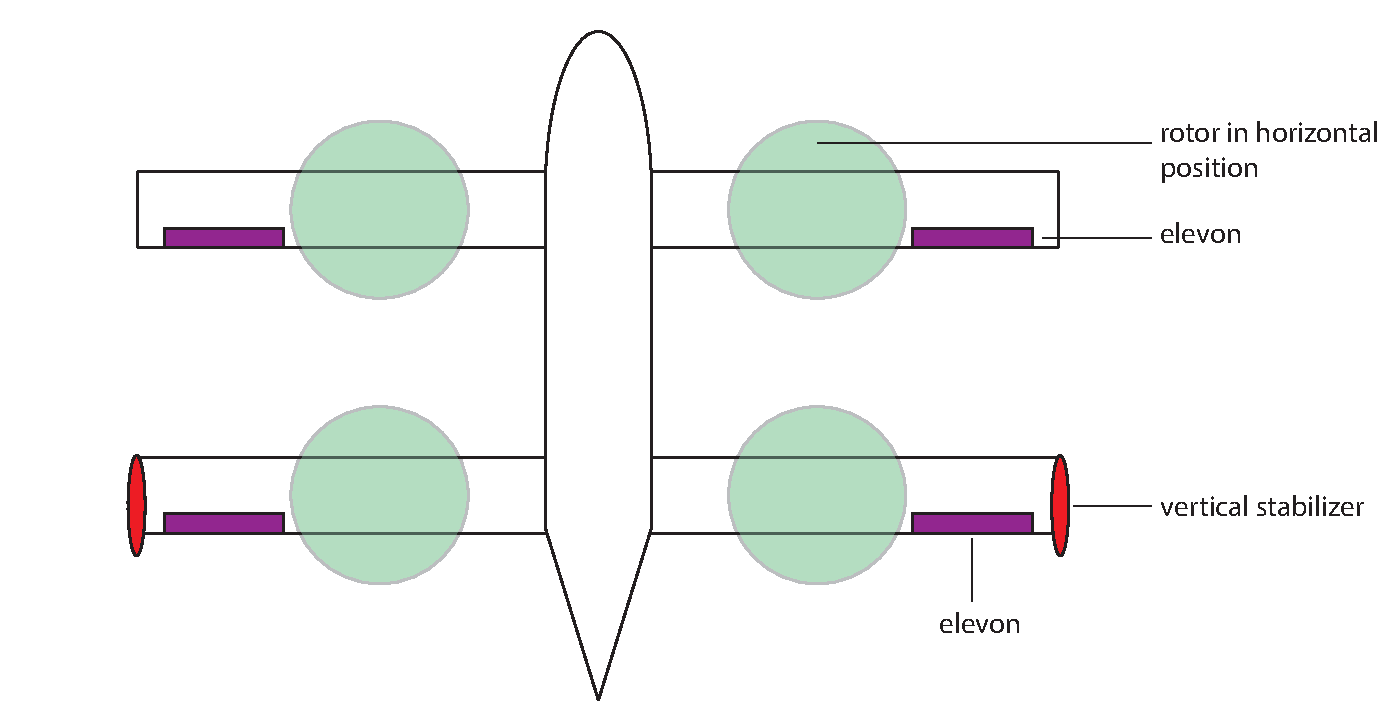
\includegraphics[height=6cm]{Stability/Figures/concept_2.pdf}
    \caption{Control Layout of The Tandem}
    \label{fig:Ctd}
\end{figure}

\paragraph{Control}
During vertical flight phases, The Tandem will be controlled in a similar way to the way conventional quadcopters are controlled. The full layout of the controls is shown in \autoref{fig:Ctd}. A total of four rotors are used to propel the craft. Two of these are rotating clockwise and the other two are rotating counter clockwise. The rotors that have the same spin direction are on the same diagonal so that they cancel out each others contribution to the rolling and pitching moments. This allows for the yaw rate to be controlled by varying the rotations speeds of both pairs. For longitudinal control, the two front and or aft engines can be throttled up or down to create the necessary control moment. Lastly, lateral control is achieved in a way analogous to the longitudinal case but with the left and right engines instead.

In horizontal flight, the wings and thereby the engines are fixed in a forward orientation. The rotors that are used for control during vertical flight are only used for propulsion in horizontal flight. The aircraft is primarily controlled with its six control surfaces. Near the tips of both wings, elevons are located to provide both longitudinal and lateral control. The winglets of the rear wing are extended upwards into vertical stabilisers that have rudders mounted on them for directional control.

Because of the reduced wingspan of the tandem wings, a greater lift imbalance is required at the locations of the elevons to generate a sufficient control moment for rolling. In order to achieve this moment, the vehicle is equipped with four of these control surfaces. Nevertheless, the generation of greater forces is also accompanied by an increased amount drag. Additionally, the shorter fuselage implies that the distance between the wings and the centre of gravity is shorter than for a conventional configuration. This requires more lift to be generated for the pitching control moment. This again is undesirable as it increases drag. During vertical manoeuvres, the UAV behaves like a quadcopter. The only difference with conventional quad copters is the increased distance between the engines, which reduces the amount of differential thrust required for pitching and rolling.

\paragraph{Manoeuvrability}
The Tandem is a very balanced concept with respect to manoeuvrability. The moment of inertia around the roll axis is average, while the values of $I_y$ and $I_z$ are on the high side compared to the other concepts. The reason for this is the placement of the engines, which are located relatively outboard, and the presence of vertical stabilisers at the wing tips.

\paragraph{Stability}
Assuming that both wings have the same airfoil, the centre of gravity should be closer to the aerodynamic centre of the front wing than that of the aft wing in order to achieve longitudinal stability. A positive change in angle of attack will cause a similar increase in lift on both wings. These increments can differ based on down wash effects and airspeed and surface area ratios between them. The slightly forward location of the centre of gravity results in a pitch down response from the aircraft since the lift from the aft wing has a longer moment arm. However, the centre of gravity position cannot be located very far in front of the midpoint between the two wings. As the centre of gravity moves forward, more lift needs to be generated by the front wing than by the aft wing. This means that heavier penalties in efficiency are paid for trimming the aircraft when the centre of gravity is shifted forward up until the limit where trimming is no longer possible. With these constraints combined, this tandem configuration comes with a very limited range of allowable CG positions. 

In vertical flight, The Tandem functions as a quadcopter. This design is neutrally stable regardless of the centre of gravity position. The moment equilibriums are kept with differential thrust on the four propellers. The rolling, pitching and yawing moments are dominated by the thrust settings and are independent of the vehicle's attitude.
% Lukas: V22
\subsection{The Tiltrotor}

\begin{figure}[htb]
    \centering
    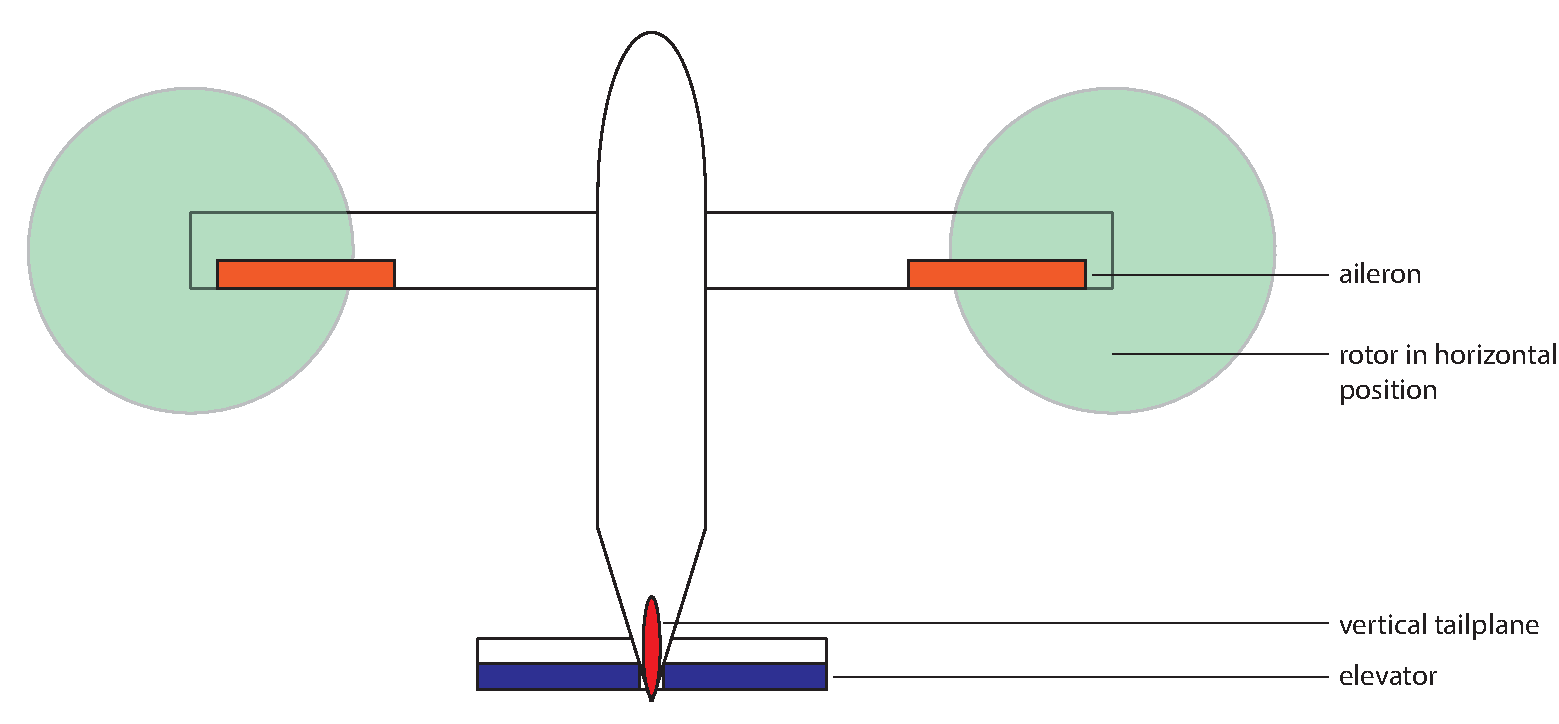
\includegraphics[height=6cm]{Stability/Figures/concept_4.pdf}
    \caption{Control Layout of The Tiltrotor}
    \label{fig:Ctr}
\end{figure}
\paragraph{Control}

The way of controlling the Tiltrotor concept was taken over from the V-22 'Osprey' transport craft and differs from both the co-axial and the three quadcopter-style designs. In \autoref{fig:Ctr} the controls of The Tiltrotor are laid out schematically.
In horizontal flight mode, The Tiltrotor relies on conventional aerodynamic control surfaces: a pair of ailerons on the main wing for roll control, elevators on the tail for pitch and a rudder for yaw. During vertical flight operations, those surfaces are ineffective, so the two engines mounted at the wing tips are used instead. Both of them can be tilted forward and backward independently and feature cyclic control swashplates\footnote{\url{http://janes.ihs.com/Janes/Display/1343214}, accessed 24-05-2017}. Pitch control is achieved by increasing the angle of attack of the forward or aft rotor blade with respect to the other one. This results in a lift asymmetry and therefore a control moment in longitudinal direction. Performing roll manoeuvres requires the collective pitch of one engines' rotor blades being different from the other one. Alternatively, the angular velocity of one engine could be varied while keeping the pitch equal, also creating a lift imbalance. Finally, yaw control in a 'helicopter mode' is done by tilting one engine forward and the other one backward. The tilted lift vectors create a net moment around the vertical axis.

The vehicle is controlled rather efficiently in horizontal flight because of the ideal layout of the control surfaces. In vertical flight phases of the mission, the attitude is controlled with the two wingtip mounted rotors. Because it will be virtually impossible to always let the centre of gravity coincide with the line connecting the two engines, a pitching moment needs to be generated by the engines to counteract the resulting thrust moment. Therefore, a continues cyclic input is usually needed in vertical flight to control the pitch angle of the UAV. 

\paragraph{Manoeuvrability}

The Tiltrotor is characterised by the two big engines located at the tips of its wing, which have a negative impact on its manoeuvrability. Especially roll performance is inferior to all other concepts due to the engine's large radius of gyration. While pitch inertia is nominal compared to the other concepts, yaw inertia also suffers from the engine placement. 

\paragraph{Stability}

In horizontal flight, The Tiltrotor is essentially a conventional configuration aircraft. The actual range of stable centre of gravity positions is dependent on a lot more detailed design considerations. However, conventional configurations are associated with relatively broad ranges of allowed centre of gravity positions. In contrast to The Tailsitter, this concept could conveniently incorporate a longer tail to increase this range even further. 

In vertical flight, The Tiltrotor is neutrally stable, as are all other concepts. The vehicle could be made laterally and longitudinally stable by implementation of a stabiliser bar of both rotors. 

% Lukas: Avy
\subsection{The Prandtl Box}
\begin{figure}[htb]
    \centering
    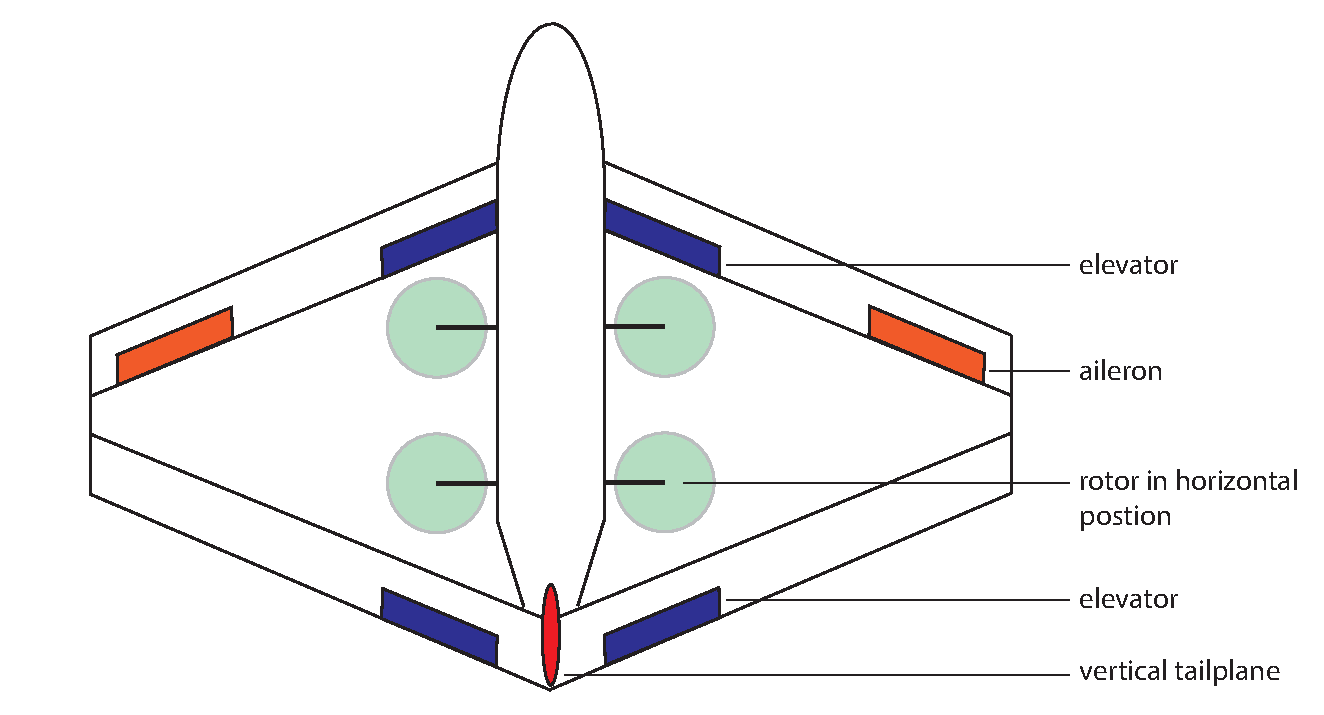
\includegraphics[height=6cm]{Stability/Figures/concept_3.pdf}
    \caption{Control Layout of The Prandtl Box}
    \label{fig:Cpb}
\end{figure}
\paragraph{Control}

The configuration of the control system of The Prandtl Box is shown in \autoref{fig:Cpb}.
From a control point of view, the Prandtl box is in many ways similar to the tandem wing. In this case, the wings are connected to each other and cannot move. Instead, the four engines are connected to the fuselage and can be tilted forward and upward. While this resembles the configuration of The Tiltrotor concept, no complex mechanisms are required for differential tilting or rotor pitch adjustments. In horizontal flight, a conventional setup was chosen for attitude control. The forward wing features two outboard ailerons for roll control, while the elevators are located on the back wing close to the body. The reason for this is the diamond shape of the wing layout, where the maximum moment arms for longitudinal control are achieved at the wing roots.
In vertical mode, the controls work similar to the ones on the tandem wing. Four pair-wise counter-rotating propellers with individual thrust settings provide pitch, roll and yaw control before being tilted for forward propulsion.

In conclusion, this concept has the same major drawback as the tandem wing configuration. The moment arms for the elevators are short in comparison to those in conventional configurations. Similar to the case of the tandem wing, this drawback is overcome by having elevators on both the front and aft wings to increase the amount of control surface area. The price to be paid for this solution is the increased trim drag caused by the greater control forces. The rudder also has a shorter moment arm, but it is used very little during flight. Therefore it's lower efficiency is acceptable. The aileron effectiveness for this concept is equivalent to that of the conventional designs since the aileron locations are as far outboard as possible while the wingspan is also similar. In vertical flight, the vehicle is essentially a quadcopter. The four rotors are positioned closer together in this design than in The Winged Quadcopter and The Tandem designs. This means that slightly more differential thrust is needed for the pitching and rolling moments. 

\paragraph{Manoeuvrability}

In terms of manoeuvrability, The Prandtl Box is comparable to The Tandem concept. The connection between the forward and backward wing introduces an extra component to the MOIs around the roll and yaw axis, however, the engines are mounted close to the body and therefore keep the MOI inertia nominal.

\paragraph{Stability}

Similar to The Tandem, The Pradtl Box has two approximately equally sized lifting surfaces. As with The Tandem, the centre of gravity should be slightly in front of the midpoint between the two wings. The aircraft can be stable about all axes. However, trimming becomes inefficient or even impossible for increasingly more forwards centre of gravity locations. 

In vertical flight, the quadcopter design renders it neutrally stable as no restoring forces are generated by any disturbance. The moment equilibriums about the vehicles axes are independent from attitude and are completely depending on the thrust of the individual propellers.

%Lukas: Jamaican cruiser
\subsection{The Winged Quadcopter}
\begin{figure}[htb]
    \centering
    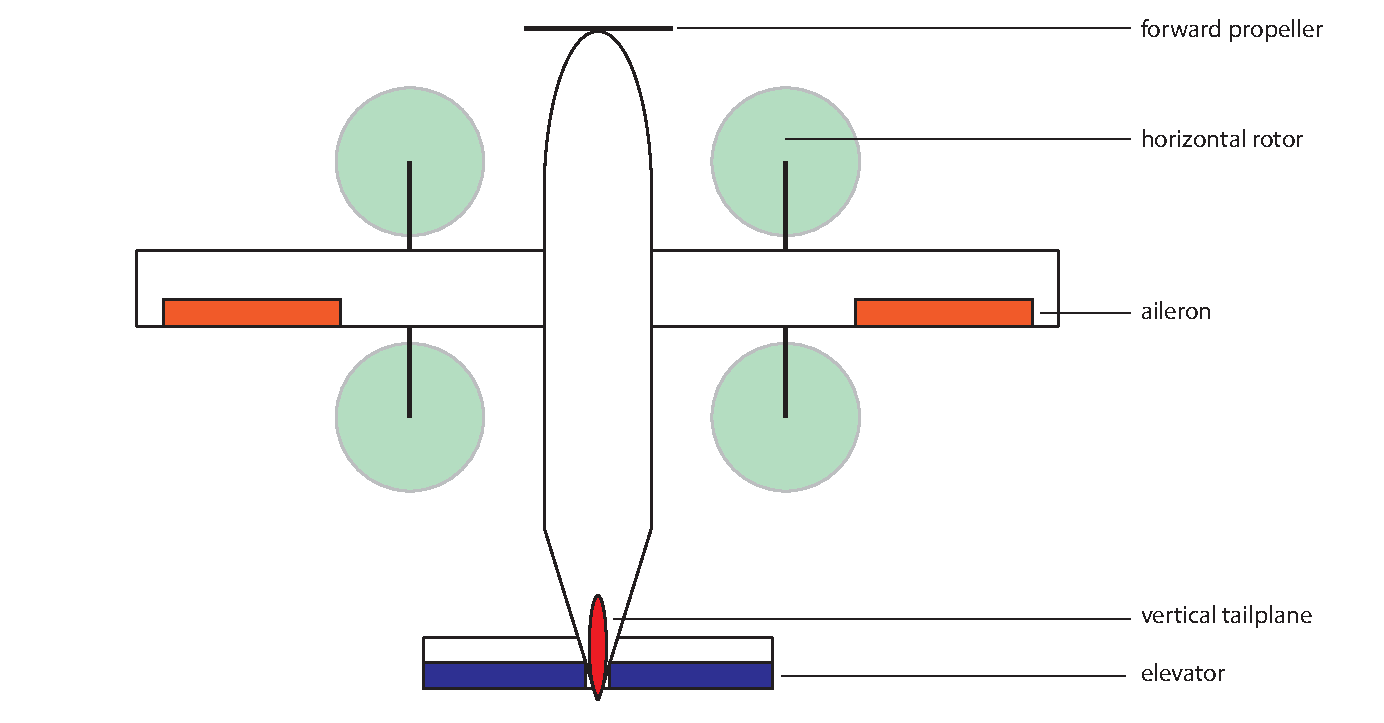
\includegraphics[height=6cm]{Stability/Figures/concept_5.pdf}
    \caption{Control Layout of The Winged Quadcopter}
    \label{fig:Cwq}
\end{figure}
\paragraph{Control}

Since this concept combines a conventional aircraft with a quadcopter, control is straightforward. The layout of the control system is depicted in \autoref{fig:Cwq}. In horizontal mode, it manoeuvres using elevators, ailerons and rudder, while in vertical mode differential thrust is applied in a fashion similar to the tandem and the Prandtl box concept. In horizontal flight, the conventional control layout results is effective and efficient control of the aircraft. In vertical flight, the quadcopter rotor configuration is also quite conventional. Only the increased distance between the rotors on the wing-mounted pylons is different. This reduces the amount of differential thrust needed for pitching and rolling control in a way analogous to The Tandem concept.

\paragraph{Manoeuvrability}

The Winged Quadcopter has a very low MOI around the roll axis, which comes close to the value The Tailsitter achieves with its central engine placement. The reason for this is the engine's placement relatively close to the fuselage, light wing and lack of wing-tip devices. Inertia values around the other two axis are the lowest of all five concepts, leading to the Winged Quadcopter being the most manoeuvrable one. 

\paragraph{Stability}

In horizontal flight, The Winged Quadcopter is no different from any other conventional configuration aircraft in terms of stability. The main wing provides most of the required lift during flight. A horizontal stabiliser at the tail provides stability for a considerable range of centre of gravity positions.
In vertical flight, The Winged Quadcopter is neutrally stable analogously to the other quadcopter designs discussed in this chapter.

